\documentclass[oneside,final,14pt,a4paper]{extreport}

\usepackage{multirow}
\usepackage[utf8]{inputenc}
\usepackage[russianb]{babel} % адаптация русского языка
\usepackage{vmargin} % настройка размера полосы набора
\setpapersize{A4}
\setmarginsrb{2cm}{2cm}{2cm}{2cm}{0pt}{0mm}{0pt}{13mm} % {левое поле}{верхнее поле}{правое поле}{нижнее поле}{колонтитулы}{колонтитулы}{колонтитулы}{номер страницы}
\usepackage{indentfirst} % отделять первую строку раздела абзацным отступом
\usepackage{graphicx} % подключение библиотеки для работы с внешними картинками
\usepackage{setspace} % для изменения межстрочного интервала
\sloppy % выравнивание текста
\setstretch{1.5} % устанавливаем межстрочный интервал

\usepackage[labelsep=space]{caption}
\addto\captionsrussian{\renewcommand{\figurename}{\CYRR\cyri\cyrs\cyru\cyrn\cyro\cyrk}} % меняем "Рис." на "Рисунок"

%\renewcommand{\thetable}{\thechapter.\arabic{table} ---} % добавить дефис после номера таблицы


\usepackage {titlesec}
\titleformat{\chapter}{\hyphenpenalty=10000\normalfont\huge\bfseries\flushleft}{\thechapter\space\space}{0pt}{\huge} % меняем заголовок для команды \chapter и запрещаем переносы слов

\usepackage{floatrow}
\floatsetup[table]{capposition=top} % разместить подпись к таблице наверху
  
\makeatletter
\renewcommand{\@biblabel}[1]{#1\space} % Заменяем библиографию с [number] на просто number:
\makeatother

\AtBeginDocument{\renewcommand\tablename{Таблица}} % переименовать Таб. на Таблица

% Начало документа
\begin{document}

\def\contentsname{Содержание} % переименовать Оглавление в содержание





% ТИТУЛЬНЫЙ ЛИСТ НАЧИНАЕТСЯ
\thispagestyle{empty}
\begin{titlepage}

\begin{figure}
	\centering
	\includegraphics[width=0.5\textwidth]{msu}\\
\end{figure}

\begin{spacing}{1.0} % устанавливаем межстрочный интервал
\begin{center} % центрируем текст
	{\small
		Московский государственный университет имени М.В. Ломоносова \\
		Факультет вычислительной математики и кибернетики \\
		Кафедра автоматизации систем вычислительных комплексов \\
	}
	\vspace{4cm}
	{\large Романов Андрей Романович \\}
	\vspace{1cm}
	{\large\bfseries
	    Разработка и реализация механизма отладки \\
	    виртуальных сетевых функций \\
	}
	\vspace{1cm}
	КУРСОВАЯ РАБОТА
\end{center}
\vfill
\begin{flushright}
\begin{small}
	{\bfseries Научный руководитель: \\}
	к.ф.-м.н. \\
	В.А. Антоненко \\
\end{small}
\end{flushright}

\vfill

\centerline{Москва, 2017}
\end{spacing}
\end{titlepage}
% ТИТУЛЬНЫЙ ЛИСТ ЗАКАНЧИВАЕТСЯ
\setcounter{page}{2}





\chapter*{Аннотация}
В данной работе рассматривается проблема отладки виртуальных сетевых функций в составе цепочек сетевых сервисов. Проведен обзор решения проблем, возникающих в компьютерных сетях, рассмотрены подходы к отладке виртуальных сетевых функций, проанализированы возможности существующих NFV платформ в части отладки виртуальных сетевых функций.

В рамках курсовой работы предложен подход к отладке виртуальных сетевых функций в рамках NFV платформы, приведено описание реализации подхода для платформы C2, проведено экспериментальное исследование производительности режима отладки.





% Оглавление
\tableofcontents % генерация оглавления





\chapter*{Введение}
\addcontentsline{toc}{chapter}{Введение} % добавление Введение в оглавление

В современных сетях функционирует достаточно большое  число сервисов: маршрутизация (routing), трансляция сетевых адресов (NAT), сетевой экран (firewall), туннелирование (VPN), защита от DDoS атак (anti-DDoS), антиспам (antispam) и многие другие. Большинство из них реализованы в одном физическом устройстве (например, маршрутизатор). В случае нехватки мощностей используют группу устройств схожей функциональности. Рекомендуется использовать устройства от одного производителя, а лучше одной и той же модели. В этом случае уменьшается риск несовместимости интерфейсов. Все это приводит к зависимости пользователей сетевого оборудования от производителя.

При возникновении необходимости в дополнительной функциональности требуется приобретать оборудование, часть функциональности которого будет избыточной. Добавление новой функциональности, исправление ошибок - это также забота команды разработчиков производителя, и пользователь в большинстве случаев не может самостоятельно вносить изменения из-за закрытости программного обеспечения оборудования. После окончания срока поддержки пользователь сетевого устройства полностью теряет возможность изменять программную составляющую. А значит необходимо приобретать новое оборудование.

Функции, реализованные в составе отдельных сетевых узлов, зачастую плохо масштабируются, так как при увеличении нагрузки на сеть увеличивается число необходимых физических устройств. При обычных (не пиковых) нагрузках часть устройств простаивает. Здесь проявляется невозможность динамического масштабирования сетевых сервисов в зависимости от загрузки.

Таким образом, можно выделить ключевые проблемы организации работы сетевых сервисов:
\begin{itemize}
	\item использование оборудования с избыточной функциональностью;
	\item расчет производительности инфраструктуры исходя из максимально возможной нагрузки;
	\item простаивание оборудования в случае, если нагрузка не является пиковой;
	\item зависимость от производителя оборудования (техническое обслуживание и устаревание оборудования, невозможность модифицировать сервис без вмешательства производителя).
\end{itemize}

Виртуализация сетевых функций позволила бы решить указанные выше проблемы, автоматизировав размещение инфраструктуры и развертывание программного обеспечения в облаке. Существует классификация в модели обслуживания облачных вычислений:
\begin{itemize}
	\item Infrastructure-as-a-Service (IaaS) -- инфраструктура как услуга;
	\item Platform-as-a-Service (PaaS) --  платформа как услуга;
	\item Software-as-a-Service (SaaS) -- программное обеспечение как услуга.
\end{itemize}

IaaS -- это модель, в которой клиенту предоставляется возможность использования облачной инфраструктуры. Пользователь сам управляет программным обеспечением предоставленных ему ресурсов. Контроль и управление физическими ресурсами облака осуществляется облачным провайдером --- поставщиком облачных услуг. Примером может служить следующие платформы: Openstack\cite{bib:openstack}, VMware Workstation\cite{bib:vmware}.

PaaS -- это модель, в которой клиенту предоставляется возможность использования платформы, предустановленной на облачной инфраструктуре. Пользователь в рамках платформы может сам определять и использовать приложения. Примером такой модели предоставления облачных услуг является платформа Google App Engine.\cite{bib:google-app-engine}

SaaS -- это модель, в которой клиенту предоставляется возможность использования программного обеспечения облачного провайдера. Отличие от PaaS заключается в том, что в SaaS клиент не может управлять сервисами облака.  Контроль и управление физическими ресурсами облака и предоставляемого программного обеспечения осуществляется облачным провайдером. Основное преимущество модели SaaS для потребителя услуги состоит в отсутствии затрат, связанных с установкой, обновлением и поддержкой работоспособности оборудования и работающего на нём программного обеспечения.

Концепцию виртуальных сетевых функций (Network Function Virtualization, NFV) возможно реализовать в виде SaaS платформы, с оговоркой, конечно, что не все сетевые функции можно эффективно виртуализировать (например, функцию маршрутизации). Это позволит решить некоторые проблемы, возникающие при эксплуатации сетевых функций. 

Программу, которая реализует концепцию NFV, обычно называют NFV платформой. Рассмотрим процесс внедрения виртуальных сетевых функций в NFV платформу. Он состоит из следующих этапов:
\begin{enumerate}
    \item разработка программного обеспечения сетевой функции (далее приложение);
    \item разработка спецификации сетевой функции;
    \item тестирование в целевой NFV платформе.
\end{enumerate}

В ходе тестирования приложения на целевой платформе разработчик сетевой функции может столкнуться с ошибками: неожиданное поведение размещенного приложения на тестовых сценариях. В случаях, когда реализованы только базовые концепции NFV платформы (см. раздел \ref{sec:nfv_description}), поиск и устранение ошибок достаточно длительный, трудоемкий, а порой и невозможный процесс. Поэтому целью данной работы является разработка механизма отладки виртуальных сетевых функций для NFV платформ.

Далее разделах \ref{sec:nfv_description}, \ref{sec:diagnosis_network_problems} подробно рассматривается концепция NFV, схема диагностики ошибок в компьютерных сетях и в NFV платформе. в разделе \ref{sec:debug_mechanism} содержатся рассуждения о том, что такое механизм отладки в NFV платформах. Затем, в разделе \ref{nfv_platform_overview} приводится обзор существующих NFV платформ. Наконец, в разделах \ref{chap:practice} и \ref{chap:expirements} приводится описание практической части и экспериментов.





\chapter{Постановка задачи}
\label{chap:problem_statement}
\section{Цель работы}
Целью данной работы является разработка механизма отладки виртуальных сетевых функций в составе цепочек (виртуальных сетевых сервисов) для NFV платформ.


\section{Задачи}
\begin{enumerate}
	\item Провести обзор существующих NFV платформ на предмет наличие в них требований к механизму отладки.
	\item Разработать механизм отладки для NFV платформ.
	\item Реализовать разработанный механизм для C2 Platform.
	\item Провести экспериментальное исследование разработанного решения.
\end{enumerate}





\chapter{Обзор предметной области}
\label{chap:overview_subject_area}



\section{Общее описание NFV}
\label{sec:nfv_description}
В традиционных сетях используется специализированное оборудование. Дорогостоящая разработка новых аппаратных решений мешает конкуренции в современных сетях, затрудняя выход на рынок новых кампаний.

Виртуализация сетевых функций (Network Function Virtualization, NFV) --- это концепция, позволяющая виртуализировать сетевые функции, которые на данный момент реализованы лишь на физических устройствах. Под виртуализацией сетевых функций понимается предоставление сетевых услуг в виде программного обеспечения, функционирующего на одной или нескольких связанных виртуальных машинах. Описание концепции NFV рассматривается на основе стандарта \cite{nfv-official}. Принципы концепции NFV:
\begin{itemize}
    \item разделение программной и аппаратной (вычислительные и сетевые ресурсы) составляющих сетевых функций;
    \item использование виртуализированной инфраструктуры для размещения сетевых функций;
    \item регистрация спецификаций сетевых функций.
\end{itemize}

NFV предполагает использование стандартных серверов и коммутаторов в качестве виртуализированной инфраструктуры для функционирования услуг. Концепция предлагает использование технологий для виртуализации функций в виде составных элементов, которые могут быть связаны для создания телекоммуникационных сервисов.

Ключевыми понятиями в концепции являются виртуальные сетевые функции (VNF) и виртуальные сетевые сервисы (VNS). VNF -- это базовые блоки, которые представляют собой спецификацию топологии, параметров инициализации, допустимых действий (action) над функцией и так далее. Заметим, что программное обеспечение, описанное в VNF должно иметь ограниченную и законченную функциональность. Не следует виртуализировать ненадежное программное обеспечение, которое не рационально использует ресурсы инфраструктуры (например, утечки памяти будут способствовать частым перезагрузкам сервиса). 

VNS -- это некоторое множество связанных между собой VNF. Обычно VNS представляется в виде цепочки VNF (VNF chaining). Последовательность функций в цепочки определяет, как будет обрабатываться трафик, попавший в этот сетевой сервис. VNS является конечной услугой, которой пользуются клиенты NFV платформы. 

Аналогию можно провести с математическим понятием функции. Пусть $x$ -- это входящие в сетевой сервис $S$ пакеты трафика. Тогда результатом работы сервиса $S$, состоящего из цепочки функций $f_{1} \to f_{2} \to f_{3}$ будет исходящий трафик $y$, такой что:
\begin{equation}
	\label{eq:service_example}
	y = f_3(f_2(f_1(x))) = S(x)
\end{equation}
В результате пакеты $x$ трансформировались в пакеты $y$, где $S$ -- это суперпозиция функций $f_{1}$, $f_{2}$, $f_{3}$. 

Таким образом, виртуальный сетевой сервис состоит из цепочки виртуальных сетевых функций, где работу каждой $i$-ой VNF можно представить в виде некоторого распределенного приложения $a_{i}$, которое обрабатывает сетевой трафик с помощью функции $f_{i}$. Цепочка таких приложений также образует некоторое абстрактное приложение $A$, которое обрабатывает трафик с помощью функции $S$. 

В ходе неправильного использования приложения $A$ или же из-за ошибок, допущенных разработчиками, может случиться, что результаты работы приложения не совпадают с ожидаемыми результатами. При детектировании таких несоответствий мы будем искать причину с помощью  алгоритма, описанного в следующем разделе.



\section{Диагностика виртуальных сетевых функций}
\label{sec:diagnosis_network_problems}

В настоящее время практически в любой компании, в которой сотрудники могут работать не только в офисе или которая состоит из нескольких филиалов, присутствует хотя бы один сетевой администратор. Его основная задача -- поддерживать корпоративную компьютерную сеть в рабочем состоянии. Возникшие неполадки в компьютерной сети (обычно по жалобе пользователей -- сотрудников компании) можно решить в кратчайшие сроки, используя алгоритм решения сетевых проблем (РСП), описанный в \cite{bib:troubleshotuin_network_problems}. Основные шаги алгоритма:
\begin{enumerate}
    \item Локализация проблемы.
    \begin{enumerate}
        \item Собрать симптомы и определить суть проблемы.
        \item Если возможно, воссоздать сбойную ситуацию.
        \item Установить причину, вызывающую сбой.
    \end{enumerate}
    \item Принять меры по решению проблемы.
    \item Провести проверку систем или оборудования, чтобы удостовериться, что проблема устранена.
    \item Задокументировать проблему и ее решение.
\end{enumerate}

Заметим, что алгоритм применим в традиционных сетях, однако неприменим для виртуализированной инфраструктуры, управляемой NFV платформой.

Проблемы возникают уже на этапе диагностирования причины сбойной ситуации. Невозможно собрать полную информацию о работе виртуальной инфраструктуры. Платформа может не обладать достаточными интерфейсами для точного определения причины. Примером может служить виртуальной сетевой сервис, в цепочке которого присутствуют виртуальные сетевые функции, доступ к которым закрыт. В этом случае невозможно определить, как закрытая функция влияет на пропускаемый трафик: сбрасывает ли она пакеты, пропускает с изменениями или без них.

В традиционных сетях истинная причина неисправности может крыться либо в аппаратной, либо в программной части. Аппаратной части в концепции NFV сопоставляется модуль управления виртуальной инфраструктурой NFV-платформы (гипервизор, подмодуль управления сетью). А программную ошибку можно рассматривать как проблему на одном из уровней сетевой модели ISO/OSI.

Опишем всевозможные ситуации, возникающие при обнаружении неполадки:
\begin{itemize}
    \item ошибки в NFV платформе;
    \item ошибки, связанные с виртуальным сетевым сервисов:
    \begin{itemize}
        \item неправильное использование;
        \item ошибки в NFV платформе (ошибки при размещении, конфигурировании и т.д.);
        \item ошибки в одной или нескольких виртуальных сетевых функциях;
        \begin{itemize}
            \item неправильное использование;
            \item ошибки в программном обеспечении виртуальной сетевой функции.
        \end{itemize}
    \end{itemize}
\end{itemize}

В предположении, что NFV платформа работает корректно, приходим к выводу, что причина неисправности всегда кроется либо в неправильном использовании, либо в программном обеспечении VNF. В первом случае достаточно внимательно прочитать документацию. Во втором --- необходимо внести изменения в программную составляющую виртуальной сетевой функции. И снова сталкиваемся с тем, что не каждая NFV платформа может предоставлять пользователю интерфейс управления размещенной инфраструктуры виртуальной сетевой функции. Поэтому в следующем разделе обсуждается требования, которым должна удовлетворять NFV платформа обладающая механизмом отладки.

\section{Механизм отладки сетевых функций}
\label{sec:debug_mechanism}

Механизм отладки виртуальных сетевых функций должен предоставлять собой удобный инструмент для диагностирования проблем с VNF. 

Механизм должен позволять быстро локализовать возникшую неполадку с точностью до экземпляра сетевой функции, что можно обеспечить за счет отображения трафика, проходящего между этими экземплярами. Такая реализация позволит экономить время при обнаружении таких проблем, как неверная конфигурация функция, неправильный классификатор у цепочки функции. Например, допустим, что виртуальная машина подписана на сетевой сервис из одной функции NAT. И было обнаружено, что на команду ''ping 8.8.8.8'', запущенной на этой виртуальной машине ,не приходят ответы ICMP reply. Тогда при просмотре трафика на входе в цепочку перед первой функцией можно обнаружить, что он не попадает в цепочку. Получается, что проблема заключается в классификаторе, в котором не указан протокол ICMP (то есть ICMP пакеты не захватываются в цепочку). 

После выяснения причины неполадки необходимо исправить ошибку. Часто ошибки заключаются либо в некорректно работающем программном обеспечении сетевой функции, либо в ее неправильной конфигурации, либо в неправильной спецификации (например, TOSCA\cite{bib:tosca}) сетевой функции. В последнем случае изменение спецификации функции может быть очень значительным и затрагивать процесс размещение и удаления сетевых функций, что не позволит корректно удалить уже существующие экземпляры. Такой процесс обновления функции является достаточно трудоемким и не будет рассматриваться в данной работе.

Таким образом, механизм отладки виртуальных сетевых функций в облачной платформе должен:
\begin{itemize}
    \item по запросу менять режим работы цепочки сетевых функций с обычного на отладочный и обратно;
    \item в режиме отладки:
    \begin{itemize}
        \item отображать трафик, проходящий между виртуальными сетевыми функциями;
        \item позволять изменять конфигурацию сетевых функций в ходе их работы;
        \item позволять вносить изменения в программное обеспечение работающей функции.
    \end{itemize}
\end{itemize}

Далее рассматриваются требования к NFV платформе, в которой возможна реализация механизм отладки виртуальных сетевых функций.





\chapter{Обзор существующих NFV платформ}
\label{nfv_platform_overview}


\section{Требования к механизму отладки}
\label{sec:debug_requirements}
Перед проведением обзора необходимо установить, по каким критериям будут сравниваться NFV платформы.

В разделе \ref{sec:diagnosis_network_problems} были описаны основные причины, по которым невозможно применить алгоритм РСП для отладки виртуального сетевого сервиса. Кратко перечислим их:
\begin{itemize}
    \item существуют ситуации, когда невозможно локализовать неисправность вплоть до уровня сетевых функций в VNS;
    \item отсутствие возможности управлять инфраструктурой VNF.
\end{itemize}

Здесь и далее в работе будем предполагать, что NFV платформа работает корректно. Это означает, что реализация возможностей платформы полностью совпадает с прилагаемой документацией.

Для решения первой проблемы достаточно, чтобы NFV платформа позволяла:
\begin{itemize}
    \item перехватывать сетевой трафик между экземплярами виртуальных сетевых функций;
    \item производить разбор сетевого трафика вплоть до 4-ого уровня модели ISO/OSI.
\end{itemize}

В этом случае, независимо от возникшей неполадки, можно всегда с уверенностью сказать, где возникла проблема с точностью до конкретной VNF в составе цепочки.

Топология виртуальной сетевой функции обычно представляет собой граф из виртуальных машин. Иногда в топологию добавляются такие элементы, как виртуальный маршрутизатор, коммутатор или же добавляется элемент виртуальная сеть. Однако все эти узлы (кроме виртуальных машин) реализуются внутри платформы. Поэтому для решения второй проблемы достаточно предоставить удаленный доступ к виртуальным машинам топологии сетевых функций. Обычно такой доступ реализован с помощью системы VNC (Virtual Network Computing\cite{bib:vnc}).

Таким образом, будем говорить, что в NFV платформе возможно реализовать механизм отладки виртуальных сетевых сервисов, если в ней реализованы следующие возможности (принципы):
\begin{itemize}
    \item перехватывается сетевой трафик между виртуальными сетевыми функциями;
    \item производиться разбор сетевого трафика вплоть до 4-ого уровня модели ISO/OSI;
    \item предоставляется удаленный доступ к виртуальным машинам топологии сетевых функций.
\end{itemize}

Перечисленные принципы позволяют диагностировать и исправить возникший сбой в VNS не выходя за возможности NFV платформы.

Теперь можно перейти к обзору самих NFV платформ. Цель обзора -- выявить такие платформы, в которых реализован механизм отладки виртуальных сетевых сервисов. В качестве критериев обзора выбраны вышеуказанные принципы механизма отладки.

% Критерии обзора должны быть такими, чтобы позволить диагностировать и исправить возникший сбой в VNS не выходя за возможности NFV платформы. В разделе \cite{sec:diagnosis_network_problems} было выявлено, что возможностей, которыми должна обладать любая NFV платформа, недостаточно для использования алгоритма РСТ.


% выяснить достоинства и недостатки существующих решений и сформировать требования к разрабатываемому решению. Решения будут сравниваться по следующим критериям:
% \begin{itemize}
%     \item TODO
% 	\item Соответствие архитектуры платформы стандарту ETSI NFV MANO.
% 	\item Независимость от платформы виртуализации ресурсов. Данный пункт означает, что решение использует программную прослойку (адаптер) для взаимодействия с платформой виртуализации. При необходимости использовать другую платформу достаточно заменить программную прослойку без переписывания кода основных модулей.
% 	\item Поддержка работы с несколькими VIM одновременно. Решение, обладающее данным свойством, способно управлять несколькими платформами виртуализации ресурсов одновременно (один модуль VIM для одной платформы виртуализации).
% 	\item Мониторинг состояния виртуального сетевого сервиса. Поддержка этого свойства позволяет следить за состоянием инфраструктуры виртуальных сетевых сервисов.
% 	\item Автоматическое срабатывание обработчиков scaling и healing. Scaling -- событие, связанное с масштабированием сервиса, healing -- событие, связанное с некорректной работой сервиса. Решение, в котором реализован данный пункт, может автоматически запускать обработчики на события scaling и healing, чтобы восстановить работу сервиса. Обработчики на события присутствуют в описании виртуальной сетевой функции.
% \end{itemize}

% Выполнение всех критериев, указанных выше, позволит решению выполнять задачи по управлению виртуальными сетевыми сервисами и обеспечивать их отказоустойчивость и масштабируемость в автоматическом режиме.


\section{Open Platform for NFV}
Open Platform for NFV (OPNFV) --- это платформа с открытым исходным кодом, на базе которой можно создавать компоненты  идеологии NFV. Проект OPNFV фокусируется на разработке менеджера инфраструктуры (NFVI) архитектуры ETSI NFV MANO\cite{opnfv-official}. Основные цели проекта:
\begin{itemize}
	\item разработка интегрированной и протестированной открытой платформы, которая может быть использована для построения NFV, ускорения внедрения новых продуктов и сервисов;
	\item привлечение заинтересованных лиц со стороны конечных заказчиков для удовлетворения требований пользовательского сообщества;
	\item создание экосистемы NFV решений, основанной на открытых стандартах и программном обеспечении, которое удовлетворяет требованиям конечных пользователей;
	\item продвигать OPNFV как предпочтительную платформу и сообщество для создания NFV решений с открытым кодом.
\end{itemize}

OPNFV стремится участвовать в смежных открытых проектах, которые могут быть использованы в OPNFV для обеспечения целостности, высокой производительности и функциональной совместимости компонентов. OPNFV активно взаимодействует с открытыми проектами: OpenStack, KVM, Open vSwitch, OpenDaylight, ONOS, Open Contrail, ETSI, IETF. Сообщество состоит из более чем 60 компаний, начиная с производителей оборудования и заканчивая поставщиками SDN и NFV решений.\cite{opnfv-state1}

Первый релиз (Arno) состоялся в июне 2015 года и какой-либо функциональности в себе не нес.
Вторая версия проекта OPNFV (Brahmaputra) вышла 1 марта 2016 года. По словам сообщества, в платформе были реализованы поддержка тестирования производительности и другие средства проверки соответствия между требованиями приложений виртуальных сетевых функций и возможностями инфраструктуры. Таким образом, платформа готова для проведения лабораторных тестов. Также упоминается о возможностях по обнаружению и устранению неисправностей в виртуальных сетевых цепочках, однако автору удалось найти в сети интернет упоминания о планах проекта OPNFV по реализация тестирования и отладки сервисных цепочек с пометкой $TODO$\cite{bib:opnfv_testing_todo}.

Как уже было отмечено, OPNFV -- это база для реализации продуктов на базе ETSI NFV MANO. В данной платформе разрабатывается лишь модуль NFVI, отвечающий за виртуальные ресурсы. Поэтому говорить о виртуальных сетевых функциях, а тем более о их отладке в рамках проекта OPNFV не приходится.


\section{Cloudify}
Cloudify -- это платформа с открытым исходным кодом. Платформа архитектурно состоит из основного модуля, называемого Cloudify Manager VM, и Cloudify агентов, установленных на подконтрольных виртуальных машинах. 

Cloudify Manager VM исполняет роли сразу двух основных модулей -- это VNFM и NFVO. Таким образом, указанный модуль выполняет множество задач:
\begin{itemize}
	\item Регистрация новых виртуальных функций. Описание функций представляется в формате собственной разработки, называемый blueprints. Он основан на стандарте описания функций TOSCA\cite{bib:tosca}.
	\item Размещение инфраструктуры VNF, используя плагины к существующим платформам виртуализации ресурсов (поддерживаются Openstack, VMware).
	\item Инициализация инфраструктуры функций. Используются программы-агенты на подконтрольных виртуальных машинах.
	\item Мониторинг изменения состояния виртуальных сетевых функций с помощью агентов.
	\item Запуск обработчика события из описания функции.
\end{itemize}

Cloudify агенты ответственны за выполнения команд от Cloudify Manager VM. Различают агентов со стороны Cloudify менеджера (manager side agents) и со стороны виртуальной сетевой функции (application side agents). Агенты менеджера устанавливаются вместе с операционной системой виртуальной машины и выполняют следующие служебные задачи: создание виртуальной машины, привязка внешнего ip-адреса и т.д.. Агенты виртуальной функции являются опцией (устанавливаются, если стоит соответствующая запись в описании функции). Задачи, выполняемые агентами функции, должны присутствовать в описании функции.\cite{cloudify-official-oveview1}

Анализ платформы Cloudify показал, что невозможно реализовать отладку виртуальных сетевых функций из-за отсутствия возможностей по перехвату трафика. 

\section{OpenStack Tacker}
Openstack Tacker -- это проект с открытым исходным кодом. Является дополнительным модулем для платформы виртуализации Openstack. Использует разработки проекта OPNFV. Основной целью проекта является реализация основных блоков ETSI NFV MANO (VNF-Manager и VNF-Orchestrator) в виде плагина для платформы виртуализации Openstack. Openstack Tacker реализует управление виртуальными сетевыми функциями и оркестрацию виртуальных сетевых сервисов.
	Рассмотрим основную функциональность базовых блоков архитектуры ETSI NFV MANO в рамках проекта Openstack Tacker. Основные задачи, выполняемые блоком VNF-Manager:
\begin{itemize}
	\item хранилище всех виртуальных функций, доступных системе;
	\item управление полным жизненным циклом каждой виртуальной функции (размещение, инициализация, масштабирование, остановка, удаление);
	\item мониторинг за размещенными виртуальными функциями. Основные параметры мониторинга: производительность и отказоустойчивость функции;
	\item автоматическое восстановление работы функции в случае ее полного или частичного отказа в предоставлении услуги по заданным политикам;
	\item облегчение первоначальной настройки виртуальной сетевой функции.
\end{itemize}

Задачи, выполняемые блоком VNF-Orchestrator:
\begin{itemize}
	\item использование шаблонов при управлении сетевыми сервисами, комбинирование различных виртуальных сетевых функций между собой;
	\item обеспечение эффективного размещения виртуальных функций;
	\item создание цепочек виртуальных сетевых функций (сетевые сервисы);
	\item контроль за выделением ресурсов с помощью блока VIM;
	\item оркестрация виртуальных сетевых функций на множестве различных блоков VIM.
\end{itemize}

На текущий момент возможности Tacker реализованы только в режиме командной строки и не доступны в графическом интерфейсе Horizon платформы Openstack.\cite{tacker-official}

Восстановление работы функции и расширение инфраструктуры функции доступно только в ручном режиме. Интеграция с платформой виртуализации Openstack не позволяет использовать другие средства виртуализации инфраструктуры. Информации по отладке виртуальных сетевых функций в платформе, как и возможностей по перехвату трафика, найдено не было.


\section{OpenBaton}
OpenBaton -- это проект с открытым исходным кодом, реализующий архитектуру ETSI NFV MANO. Основными модулями платформы являются:
\begin{itemize}
	\item оркестратор виртуальных сетевых сервисов NFVO;
	\item менеджер виртуальных сетевых функций VNFM;
\end{itemize}

Основным модулем, над которым ведется разработка --- NFVO. В нем содержится основная функциональность: размещение функций, слежение за их состоянием, восстановление из аварийного состояния и масштабирование. VNFM является заменяемым модулем: возможно использование модуля управления функциями собственной разработки. При этом с OpenBaton поставляются библиотеки, позволяющие упростить разработку и интегрирование собственного VNFM с оркестратором NFVO.

OpenBaton независима от платформы виртуализации ресурсов. На текущий момент разработан только плагин под платформу Openstack. Разработчиками заявлена поддержка одновременной работы с несколькими VIM. В OpenBaton для включения функции мониторинга необходимо дополнительно установить Zabbix сервер (о поддержке других решений по слежению за виртуальными машинами автору не известно).

На момент написания работы в OpenBaton идет разработка следующей функциональности: развертывания дополнительной инфраструктуры и разнообразные улучшения в blueprints. Из этого следует, что о реализации автоматического масштабирования и восстановления функции речи пока не идет.

Для реализации собственных виртуальных сетевых сервисов OpenBaton предлагает либо реализовать менеджер функций собственной разработки, либо привести описании функции через VNFPackage. VNFPackage -- это описание функции на основе формата YAML, который содержит необходимое описание виртуальной сетевой функции.\cite{bib:openbaton-official}

В документации к платформе также не было найдено какой-либо информации по отладке виртуальных сетевых функций. В платформе не уделяется внимание перехвату трафика, так необходимого для реализации механизма отладки.


\section{Проприетарные решения}
Автору не известны проприетарные решения, реализующие концепцию NFV. Наиболее популярные продукты Microsoft Azure и VMware vSphere работают в рамках модели IaaS. Указанные платформы можно использовать только в качестве менеджера инфраструктуры в рамках архитектуры ETSI NFV MANO.


\section{Выводы}
Результаты обзора показали, что ни одно из обозреваемых решений не обладает механизмом отладки. В таблице \ref{tab:nfv_platform_comprassion} приведено наличие требований механизма отладки для каждой NFV платформы.

\renewcommand{\arraystretch}{1.5}
\begin{table}[h]
\center % центрирование таблицы
\begin{tabular}{|p{0.2\textwidth}|p{0.2\textwidth}|p{0.2\textwidth}|p{0.2\textwidth}|p{0.2\textwidth}|p{0.2\textwidth}|} % разделить колонки вертикальными линиями и центрировать содержимое каждой колонки
\hline % прочертить горизонтальную линию
Плат\-фор\-ма & Перехват трафика между VNF & Разбор трафика до уровня L4 ISO/OSI & Удаленный доступ к виртуальным машинам VNF \\
\hline
OPNFV & - & - & + \\
\hline
Cloudify & - & - & + \\
\hline
Openstack Tacker & - & - & + \\
\hline
%CORD on.lab & & & & & \\
%\hline
OpenBaton & - & - & + \\
\hline
%vSphere & ? & ? & ? & ? & ? \\
%\hline
%Azure & ? & ? & ? & ? & ? \\
%\hline
\end{tabular}
\caption{--- Сравнение NFV платформ.}
\label{tab:nfv_platform_comprassion}
\end{table}






\chapter{Требования к решению}
\label{sec:platform_requirements}
На основании результатов обзора и на основании анализа механизма отладки сетевых функций из раздела \ref{sec:debug_mechanism} сформулируем требования, которым должно удовлетворять разрабатываемое решение. Итак, механизм отладки виртуальных сетевых функций в NFV платформе должен:
\begin{itemize}
    \item по запросу менять режим работы цепочки сетевых функций с обычного на отладочный и обратно;
    \item в режиме отладки:
    \begin{itemize}
        \item отображать трафик, проходящий между виртуальными сетевыми функциями;
        \item позволять изменять конфигурацию сетевых функций в ходе их работы;
        \item позволять вносить изменения в программном обеспечении работающей функции;
    \end{itemize}
\end{itemize}





\chapter{Описание практической части}
\label{chap:practice}
В текущей главе приведено описание реализации механизма отладки виртуальных сетевых функций для платформы C2 Platform\cite{bib:c2_platform}. Проект разрабатывается отечественной организацией Центр Прикладных Исследований Компьютерных Сетей (ЦПИКС).

\section{Облачная платформа C2 Platform}
\label{sec:c2-platform-description}
Рассматриваемая NFV платформа реализована по высокоуровевой архитектуре ETSI NFV MANO. Взаимодействие между внутренними модулями оуществляется через библиотеку RabbitMQ (RMQ). \cite{bib:rabbitmq}

Проект C2 Platform состоит из нескольких модулей:
\begin{itemize}
	\item веб-интерфейс платформы (GUI-сlient);
	\item модуль, предоставляющий интерфейс для OSS/BSS систем (GUI-server);
	\item модуль виртуализации инфраструктуры (VIM);
	\item модуль мониторинга (Mon);
	\item менеджер функций (VNFM, в разработке);
	\item оркестратор сервисов (Orch, в разработке);
\end{itemize}

Далее представлено подробное описание модулей платформы C2.

\subsection{Графический интерфейс}
Оба модуля (GUI-client и GUI-server) отвечают за:
\begin{itemize}
	\item отображение актуальной информации о текущей загрузке физических серверов;
	\item отображение размещенных тенантов (тенант -- это сети виртуальных машин);
	\item авторизацию пользователей;
	\item предоставление управления виртуальными сетевыми функциями и виртуальными сетевыми сервисами;
	\item отображение актуального состояния сетевых функций и сервисов.
\end{itemize}

Модуль GUI-server является поставщиком данных для GUI-client. В нем сосредоточены все основные интерфейсы платформы C2. 

\subsection{Модуль виртуализации ресурсов}
Модуль VIM состоит из двух основных частей: плагин для существующей платформы виртуализации ресурсов (используется Openstack) и независимая часть для обработки сообщений от других модулей проекта C2 Platform (Mon, VNFM, GUI-server и т.д.). Плагин можно менять в зависимости от используемой платформы виртуализации ресурсов (Openstack, VMWare и т.д.). Задача второй части заключается в управлении тенантами (сеть с виртуальными машинами) по запросу от других модулей платформы. 

Основные интерфейсы для других модулей: размещение и удаление тенанта, предоставление консоли к конкретной виртуальной машине, предоставление информации о размещенных сетях и виртуальных машинах, информация о занятых ресурсах, реализация цепочки сетевых функций и т.д..

\subsection{Модуль мониторинга}
Модуль мониторинга Mon так же состоит из двух частей: плагин для существующей программы мониторинга (используется Zabbix \cite{bib:zabbix}) и независимая часть для обработки сообщений от других модулей проекта C2 Platform (GUI-server, VNFM, и т.д.). Плагин можно менять в зависимости от используемой программы мониторинга. Независимая часть обеспечивает слежение за виртуальными машинами, соединениями между ними.

Основные интерфейсы для других модулей: установка и удаление мониторов за виртуальными машинами, оповещение подписанных модулей о событиях, предоставление статистики по работе виртуальных машин.

\subsection{Модуль оркестрации сервисов}
Модуль оркестрации виртуальных сетевых сервисов Orch занимается размещением, переконфигурации цепочек сетевых функций, отправляя запросы к модулям VIM и VNFM. Имея возможность взаимодействовать сразу с несколькими модулями VIM, оркестратор, исходя из текущей загруженности доступных ЦОД, решает, куда необходимо разместить очередную цепочку. В текущей реализации имеется возможность размещать одну цепочку сетевых функций на инфраструктуре одного виртуального ЦОД (инфраструктурой одного виртуального ЦОД управляет один модуль VIM).

Основной интерфейс, предоставляемый модулем: размещение, удаление, переконфигурирование виртуальных сетевых сервисов.

\subsection{Модуль управления виртуальными сетевыми функциями}
Модуль управления виртуальными сетевыми функциями VNFM состоит из двух основных частей: анализатор описания виртуальных сетевых функций и часть для взаимодействия с другими модулями проекта C2 Platform (Orch, VNFM). Модуль умеет регистрировать виртуальные сетевые функции, внося соответствующую информацию в базу данных. Модуль анализирует описание функции и занимается конфигурацией ее инфраструктуры.

Основной интерфейс, предоставляемый модулем: управление, конфигурирование и поддержка виртуальных сетевых функций.


\section{Реализация механизма отладки}
\label{sec:developed_module}
Механизм отладки был реализован в модуле GUI-server, так как он предоставляет интерфейс для OSS/BSS систем и для администраторов облачной платформы.
В дополнении к остальным интерфейсам модуля была добавлена возможность включать и выключать режим отладки для цепочки сетевых функций. В ходе запроса используется одна из существующих виртуальных сетевых функций, зарегистрированных в платформе, которая осуществляет перехват трафика. Будем называть эту VNF отладочной. В процессе запроса на переход в отладочный режим выполняются следующие действия:
\begin{enumerate}
    \item проверка существования отладочной VNF;
    \item редактирование структуры цепочки целевого сетевого сервиса;
    \item производится размещение дополнительных отладочных VNF;
    \item обновление цепочки сетевого сервиса.
\end{enumerate}

В результате мы получаем цепочку сетевых функций, в которой на четных позициях (нумерация с нуля) располагаются отладочные VNF. Для возможности перехода в отладочный режим без удаления существующих функций была добавлен интерфейс переконфигурирования виртуального сетевого сервиса в модуле Orch. Переконфигурация означает изменения структуры цепочки сетевых функций, в ходе которой добавляются новые экземпляры, удаляются старые и не изменяются существующие VNF. На рисунке \ref{pic:orch_classes_diagram} представлена диаграмма классов модуля Orch. Разработанный интерфейс переконфигурации сетевого сервиса соответствует пункту $reconfigure\_handler()$ в блоке $GUIManager$.
\begin{figure}[h]
	\centering
	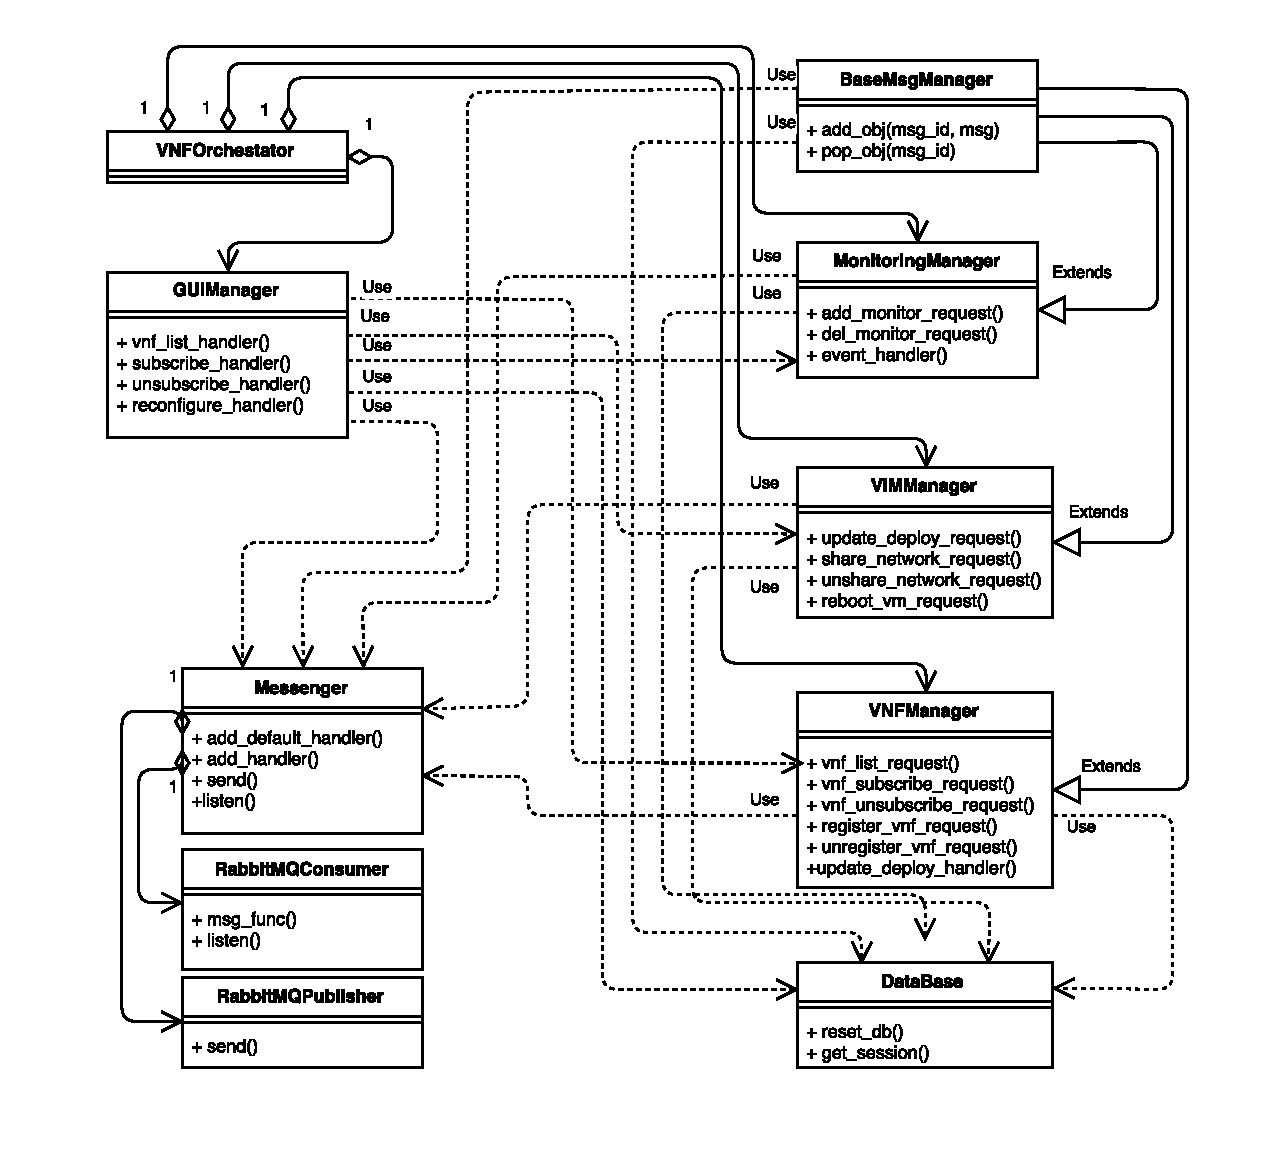
\includegraphics[width=0.95\textwidth]{orch_classes_diagram}
	\caption{--- Диаграмма классов модуля Orch}
	\label{pic:orch_classes_diagram}
\end{figure}

Как было упомянуто, интерфейс перехода виртуального сетевого сервиса в отладочный режим был реализован в модуле GUI-server. На рисунке \ref{pic:guis_classes_diagram} представлена диаграмма классов модуля GUI-server. Разработанный интерфейс $debug\_mode()$ можно увидеть в блоке $ClientManager$.
\begin{figure}[h]
	\centering
	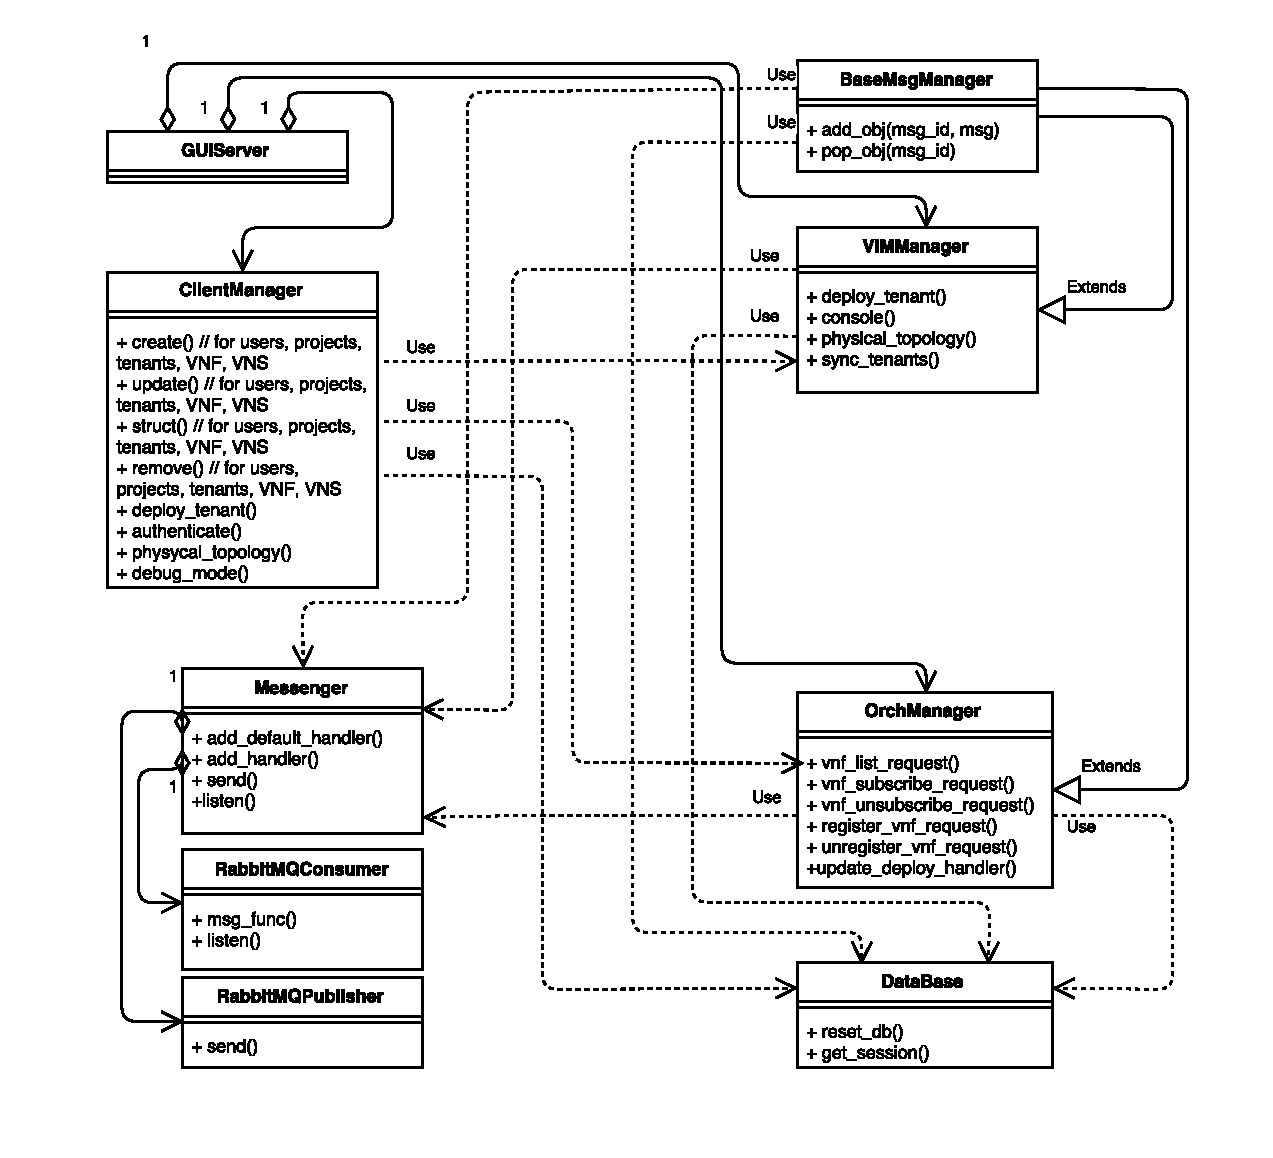
\includegraphics[width=0.95\textwidth]{gui_classes_diagram}
	\caption{--- Диаграмма классов модуля GUI-server}
	\label{pic:guis_classes_diagram}
\end{figure}





\chapter{Экспериментальные исследования}
\label{chap:expirements}
В данной главе представлено описание экспериментального исследования разработанного режима отладки для платформы C2. Цель экспериментов --- исследовать, как режим отладки влияет на время между отправкой запроса и получением ответа (RTT) в случае, когда трафик проходит через виртуальный сетевой сервис. А также измерить, сколько дополнительных ресурсов необходимо для работы сетевой функции в режиме отладки.

В платформе C2 отладочная VNF представляется в виде образа дистрибутива Ubuntu версии 15.10 с предустановленным приложением wireshark\cite{bib:wireshark}. Данная сетевая функция требует виртуальную машину со следующими характеристиками: 1 ядро процессора (CPU), 1024 Мбайт оперативной памяти (RAM), 20 Гбайт пространства на диске (DISK). Таким образом, захват трафика происходит средствами отладочной функции. Пользователь, проводящий отладку, может получить VNC к виртуальной машине с приложением wireshark и произвести мониторинг трафика. 


\section{Описания экспериментов}
Эксперименты проводились с виртуальной сетевой функцией suricata\cite{bib:suricata} --- системой предотвращения вторжений. В минимальной комплектации, указанная сетевая функция требует единственную виртуальную машину со следующими характеристиками: 1 ядро процессора (CPU), 1024 Мбайт оперативной памяти (RAM), 10 Гбайт пространства на диске (DISK). В качестве образа используется Ubuntu с предустановленным приложением suricata.

Предполагается, что в платформе зарегистрирована виртуальная сетевая функция suricata с вышеописанными характеристиками. Также, предполагается, что в платформе уже размещен виртуальный сетевой сервис suricata, на который подписаны две виртуальные машины vm1 и vm2. VNS размещен так, что любой трафик от vm1 к vm2, перехватывается и проходит через VNF suricata, а затем выходит из сервиса обратно в сеть. На рисунке \ref{pic:subscriber_tenant} изображен описанный пользовательский тенант, размещенный в платформе С2. 

\begin{figure}[h]
	\centering
	\includegraphics[width=0.95\textwidth]{subscriber_tenant}
	\caption{--- Пользовательский тенант}
	\label{pic:subscriber_tenant}
\end{figure}

Для проверки RTT используется команда на виртуальной машине vm1 "ping vm2 -c 10". Эксперименты проводились с VNS, состоящими исключительно из VNF suricata. Использовались следующие длины цепочек: 1, 3, 5, 10. Также при проведении экспериментов отдельно анализировалось, сколько ресурсов было потрачено на работу сервиса в нормальном режиме и в режиме отладки.


\section{Результаты}
После проведения экспериментального исследования были получены следующие результаты: в таблицах \ref{tab:normal_experimental_results} и \ref{tab:experimental_results} приведены полученные экспериментальные данные о работе виртуальных сетевых сервисов, функционирующих в нормальном и отладочном режиме соответственно. Согласно результатов сетевой функции suricata требуется около 150\% ресурсов дополнительно для функционирования в режиме отладки. Заметим, что объем дополнительных ресурсов определяется требованиями ПО отладочной функции и их количеством. Поэтому в целях экономии можно использовать менее требовательные образы для соответствующих виртуальных машин или использовать более эффективный алгоритм перевода сетевого сервиса в отладочный режим. Результаты показали, что реализованный механизм отладки более эффективно использует ресурсы (по отношению к затратам на саму VNF) на ''толстых'' виртуальных сетевых функциях, когда расход ресурсов на отладочную VNF незначителен по отношению к отлаживаемой VNF.

Также необходимо отметить, что механизм отладки мало влияет на время отклика сетевого сервиса (RTT изменяется незначительно), однако на достаточно большом количестве функций (> 100) задержка может быть значительной. На практике автору не встречались случаи использования сетевых сервисов такого размера.

\renewcommand{\arraystretch}{1.5}
\begin{table}[h]
\center % центрирование таблицы
\begin{tabular}{|p{0.1\textwidth}|p{0.1\textwidth}|p{0.1\textwidth}|p{0.1\textwidth}|p{0.1\textwidth}|p{0.1\textwidth}|p{0.1\textwidth}|} % разделить колонки вертикальными линиями и центрировать содержимое каждой колонки
\hline % прочертить горизонтальную линию
\multirow{2}{1}{Длина цепочки} & \multicolumn{3}{c|}{RTT (мс)} & \multicolumn{3}{c|}{Затраты ресурсов} \\
\cline{2-7}
& min & avg & max & CPU (кол.) & RAM (Мбайт) & DISK (Гбайт) \\
\hline
1 & 58.1 & 59.1 & 68.8 & 1 & 2048 & 10 \\
\hline
3 & 58.0 & 59.2 & 61.9 & 3 & 6144 & 30 \\
\hline
5 & 59.0 & 59.4 & 64.3 & 5 & 10240 & 50 \\
\hline
10 & 59.2 & 60.0 & 70.0 & 10 & 20480 & 100 \\
\hline
\end{tabular}
\caption{--- VNS в нормальном режиме.}
\label{tab:normal_experimental_results}
\end{table}


\renewcommand{\arraystretch}{1.5}
\begin{table}[h]
\center % центрирование таблицы
\begin{tabular}{|p{0.1\textwidth}|p{0.1\textwidth}|p{0.1\textwidth}|p{0.1\textwidth}|p{0.1\textwidth}|p{0.1\textwidth}|p{0.1\textwidth}|} % разделить колонки вертикальными линиями и центрировать содержимое каждой колонки
\hline % прочертить горизонтальную линию

\multirow{2}{1}{Длина цепочки} & \multicolumn{3}{c|}{RTT (мс)} & \multicolumn{3}{c|}{Затраты ресурсов} \\
% \multirow{ 2}{*}{1} & 0 & 6 & 230 & 35 & 40 & 55 & 25 & 40 & 35 & \
\cline{2-7}
& min & avg & max & CPU (кол.) & RAM (Мбайт) & DISK (Гбайт) \\
% & \multicolumn{3}{c|}{RTT (мс)} & \multicolumn{3}{c|}{ресурсы для режима debug} \\

% \multirow{3}{*}{Длина цепочки} 
\hline
1 & 57.3 & 59.3 & 61.0 & 3 & 4096 & 30 \\
\hline
3 & 58.6 & 59.5 & 64.9 & 7 & 10240 & 80 \\
\hline
5 & 58.9 & 60.1 & 62.2 & 11 & 16384 & 170 \\
\hline
10 & 59.5 & 60.5 & 63.8 & 21 & 31744 & 320 \\
\hline
\end{tabular}
\caption{--- VNS в режиме отладки.}
\label{tab:experimental_results}
\end{table}





\chapter*{Заключение}
\addcontentsline{toc}{chapter}{Заключение} % добавить Заключение в оглавление
В рамках данной работы был предложен механизм отладки виртуальных сетевых функций для NFV платформ.

В разделе \ref{sec:diagnosis_network_problems} был проведен анализ ошибок, которые возникают при внедрении виртуальных сетевых функций в NFV платформу, и сформированы требования к механизму отладки. Затем, в разделе \ref{nfv_platform_overview} представлен обзор существующих решений, который показал, что на текущий момент не существует механизма отладки виртуальных сетевых функций для NFV платформ. Поэтому был предложен собственный механизм отладки, реализация которого представлена в разделе \ref{chap:practice}. Наконец, в разделе \ref{chap:expirements} приведено экспериментальное исследование производительности разработанного решения для платформы C2.

Разработанное решение позволяет проводить отладку виртуальной сетевой функции в рамках целевой NFV платформы. В механизме отладки нуждается любая NFV платформа, так как он позволяет проводить внедрение новый сетевых функций без необходимости связываться с разработчиками платформы.

Дальнейшие исследования в этой области могут быть направлены на оптимизацию расхода ресурсов в отладочном режиме. Также стоит рассмотреть вопрос о задании способов отладки и описании механизма тестирования VNF с помощью языка спецификации виртуальных сетевых функций (например, TOSCA).





% Список литературы
\begin{thebibliography}{00}
\addcontentsline{toc}{chapter}{Литература}
\bibitem{nfv-official} Network Functions Virtualization; white paper; ETSI; October, 2012.
\bibitem{bib:openstack} OpenStack, OpenStack Compute Admin Manual Manual, November 2011.
\bibitem{bib:vmware} Memory Resource Management in VMware ESX Server; C. Waldspurger; Operating Systems Design and Implementation (OSDI); 2002.
\bibitem{nfv-state2} NFV для корпоративных сервисов; Сергей Орлов; Журнал сетевых решений LAN № 12; Ноябрь, 2014.
\bibitem{nfv-state1} NFV виртуализация сетевых функций (дата обращения 1 мая 2017 года) [HTML] (http://sci-article.ru/stat.php?i=1455156066).
\bibitem{opnfv-official} OPNFV - An open platform to accelerate NFV; Linux Foundation; October, 2014.
\bibitem{opnfv-state1} Чем занимается сообщество OPNFV? (дата обращения 1 мая 2017 года) [HTML] (https://sdnblog.ru/who-is-opnfv).
\bibitem{cloudify-official-oveview1} Cloudify Overwiew (дата обращения 1 мая 2017 года) [HTML] (http://getcloudify.org/guide/3.1/overview-architecture.html).
\bibitem{tacker-official} Openstack Tacker (дата обращения 1 мая 2017 года) [HTML] (https://wiki.opfirewallenstack.org/wiki/Tacker).
\bibitem{bib:openbaton-official} OpenBaton (дата обращения 1 мая 2017 года) [HTML] (http://openbaton.github.io).
\bibitem{bib:google-app-engine} Google App Engine; Alexander Zahariev; Helsinki University of Technology;  April, 2009.
\bibitem{bib:rabbitmq} ManageIQ documentation. (дата обращения 1 мая 2017 года) [HTML] (http://manageiq.org/docs)
\bibitem{bib:zabbix} R. Olups. Zabbix 1.8 Network Monitoring. Olton, Birmingham, 2010
\bibitem{bib:tosca} TOSCA Simple Profile in YAML Version 1.0; Standards Track Work Product; OASIS Open 2016; December 2016.
\bibitem{bib:c2_platform} СloudConductor: NFV платформа для реализации эталонной модели ETSI NFV MANO [HTML] (http://arccn.ru/solutions/c2\_startup/)
\bibitem{bib:troubleshotuin_network_problems} Руководство по устранению сбоев в компьютерных сетях; Fluke Network; Network Super Vision; April, 2009.
\bibitem{bib:bottrack-official} BotTrack: Tracking Botnets Using NetFlow and PageRank; Jérôme François, Shaonan Wang, Radu State, Thomas Engel; International Conference on Research in Networking; 2011.
\bibitem{bib:vnc} Virtual Network Computing Based Remote Desktop Access; Md. Sanaullah Baig, Rajasekar M., Balaji P.; International Journal of Computer Science and Telecommunications; Department of Computer Science and Engineering, Gojan School of Business and Technology, Chennai-600052, India; May 2012.
\bibitem{bib:opnfv_testing_todo} Vnf Deployment Test Cases. [HTML] (https://wiki.opnfv.org/display/PROJ/Vnf+Deployment+Test+Cases)
\bibitem{bib:wireshark} Wireshark User's Guide for Wireshark 1.11; Ulf Lamping , Richard Sharpe , Ed Warnicke; NS Computer Software and Services P/L, 2013.
Ed Warnicke,
\bibitem{bib:suricata} A Performance Analysis of Snort and Suricata Network Intrusion Detection and Prevention Engines; David J. Day Benjamin M. Burns; School of Computing and Mathematics University of Derby, Derby, UK; ICDS 2011 : The Fifth International Conference on Digital Society; 2011.
\end{thebibliography}

% Конец документа
\end{document}